\documentclass[main.tex]{subfiles}
\begin{document}

\section{December exercises}

\subsection{Exercise 10}

We have a time series of \(N\) data points, \(D = \qty{d_i}\), corresponding to the times \(t_i\), which are separated by the constant spacing \(\Delta \).

We model them as 
%
\begin{align}
d_i = \underbrace{B_1  \cos(\omega t_i) + B_2 \sin(\omega t_i)}_{f(t_i)} + n_i
\,,
\end{align}
%
where \(f(t)\) the signal we want to characterize, which depends on the unknown amplitudes \(B_1 \) and \(B_2 \) and the unknown frequency \(\omega \); while \(n_i \) is the noise: each \(n_i\) is i.i.d.\ as a zero-mean Gaussian with known variance \(\sigma^2\). 

\begin{figure}[ht]
\centering
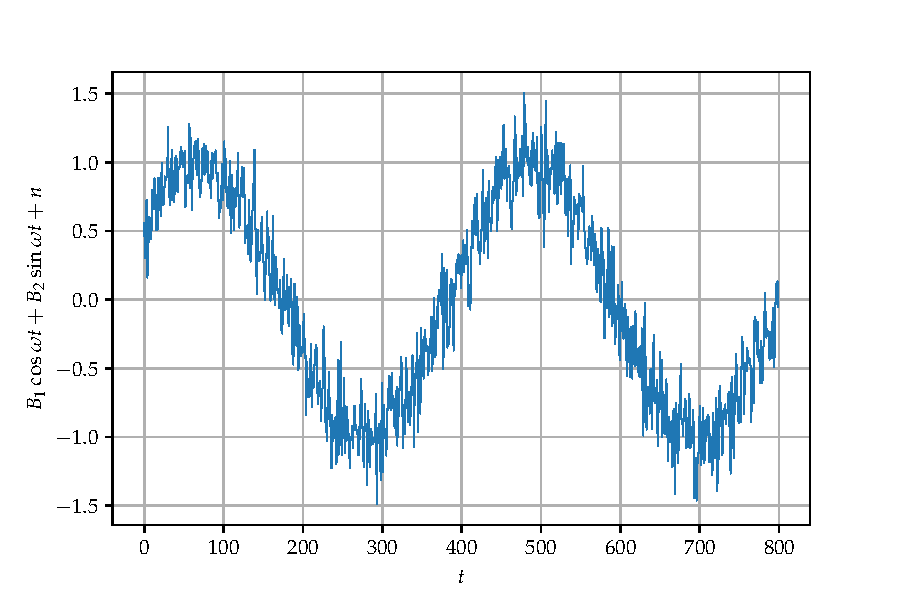
\includegraphics[width=\textwidth]{figures/signal.pdf}
\caption{Example of a portion of the signal the model assumes; the true signal should be longer than a few periods, and it is taken to be 20 times as long as this in the numerical examples which follow. The parameters are \(B_1 = 1/2\), \(B_2 = \sqrt{3} /2\), \(\sigma = 0.2\), \(\Delta = 1\), \(\omega = 0.015\).}
\label{fig:signal}
\end{figure}

\subsubsection{The full likelihood}

The likelihood of a single datum of index \(i\) attaining the value \(d_i\) is given\footnote{Omitting the dependence on previous information for simplicity.} by 
%
\begin{align}
\mathscr{L} (d_i | \omega , B_1 , B_2 ) = \frac{1}{\sqrt{2 \pi } \sigma }\exp(- \frac{1}{2 \sigma^2}\qty(d_i - f(t_i))^2)
\,.
\end{align}

Now, since the noise at each point is independent, the full likelihood is the product of the likelihoods of each datum: 
%
\begin{align}
\mathscr{L}(D | \omega , B_1 , B_2 ) &= \frac{1}{(\sqrt{2 \pi } \sigma )^{N}} \prod_{i=1}^{N} \exp(- \frac{1}{2 \sigma^2} \qty(d_i - f(t_i))^2)  \\
&= \frac{1}{(\sqrt{2 \pi } \sigma )^{N}}
\exp(- \frac{1}{2 \sigma^2} \sum_{i=1}^{N} \qty(d_i - f(t_i))^2) \\
&= \frac{1}{(\sqrt{2 \pi } \sigma )^{N}}
\exp(- \frac{1}{2 \sigma^2} \underbrace{\sum_{i=1}^{N} \qty(d_i - B_1  \cos(\omega t_i) - B_2 \sin(\omega t_i))^2}_{Q}) 
\,.
\end{align}

Let us manipulate the sum in the exponent, which we denote as \(Q\): 
%
\begin{align}
Q &= \sum _{i} d_i^2 -2 \sum _i d_i \qty(B_1  \cos(\omega t_i) + B_2 \sin(\omega t_i))
+ \sum _{i} \qty(B_1  \cos(\omega t_i) + B_2 \sin(\omega t_i))^2  \\
\begin{split}
&= N \overline{d}^2 
-2 B_1 \underbrace{\sum _{i} d_i \cos(\omega t_i)}_{R_1(\omega )}
-2 B_2 \underbrace{\sum _{i} d_i \sin(\omega t_i)}_{R_2(\omega )} + \\
&\phantom{=}\ 
+ B_1^2 \underbrace{\sum _{i} \cos^2( \omega t_i)}_{c}
+ B_2^2 \underbrace{\sum _{i} \sin^2( \omega t_i)}_{s}
+ 2 B_1 B_2 \sum _{i} \cos(\omega t_i) \sin(\omega t_i) 
\end{split}  \\
&= N \overline{d}^2 - 2 B_1 R_1(\omega ) -2 B_2 R_2(\omega ) + B_1^2 c + B_2 s + B_1 B_2 \underbrace{\sum _{i} \sin(2 \omega t_i)}_{h}
\,.
\end{align}

\subsubsection{Large pulsation limit}

The condition we ask of our signal is to have many data points for each period (\(\Delta \ll \omega^{-1}\)) and many sampled periods (\(N \Delta  \gg \omega^{-1}\)), which is equivalent to \((N \Delta )^{-1 } \ll \omega \ll \Delta^{-1} \).

The values of \(c\), \(s\) and \(h\) for various values of \(\omega \) are shown in figure \ref{fig:large_pulsation}.

\begin{figure}[ht]
\centering
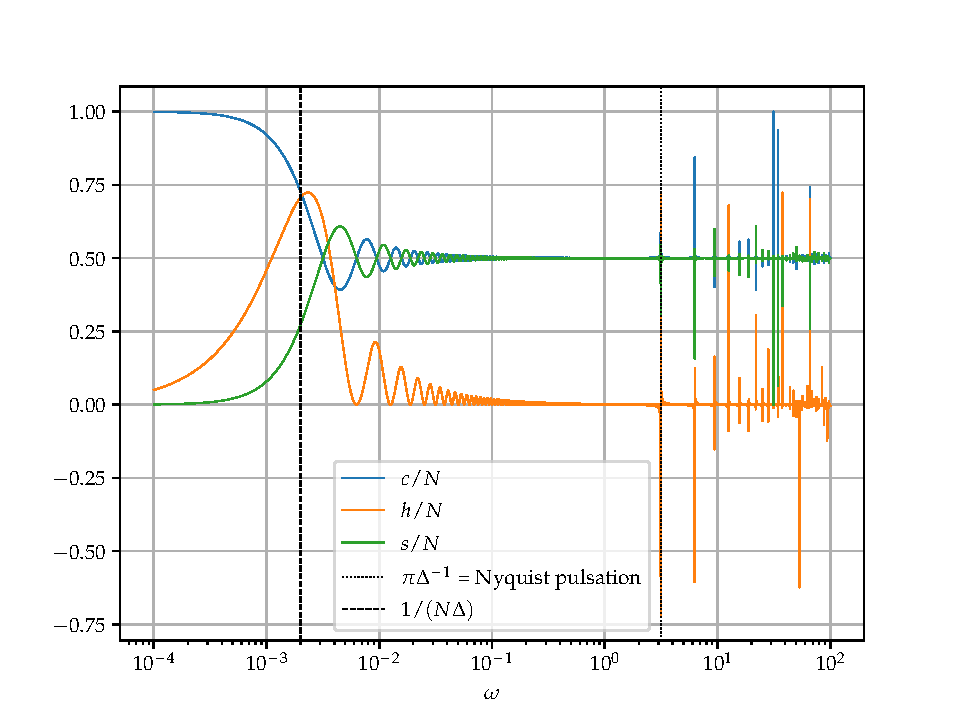
\includegraphics[width=\textwidth]{figures/large_pulsation}
\caption{Values of \(c\), \(s\) and \(h\) for different orders of magnitude of \(\omega \). The sampling frequency is fixed at \(\Delta^{-1} = 1\), and \(N=500\) points are always sampled. The conditions we ask, in the context of this plot, would mean that we put ourselves roughly in the middle of the two marked vertical lines, in the region \(\omega \sim \num{e-1}\).} 
\label{fig:large_pulsation}
\end{figure}

% However, as we can see in figure \ref{fig:large_pulsation}, the three functions do not really \emph{converge} to those values, and stating something like ``\(\lim_{\omega \to \infty } c = N /2\)'' would be incorrect mathematically.
% This is due to the presence of \emph{resonance}: if the ratio \(\omega \Delta \) is a rational multiple of \(\pi \), especially with a small denominator, there will be a bias in the points sampled, resulting in values which may range all the way from 0 to \(N\) for \(c\) and \(s\), and from \(-N\) to \(N\) for \(h\). 
% This should not really be an issue in realistic cases, as the set of points for which happens has measure zero. 

% Really, working in the \(\omega \gg \Delta^{-1}\) regime is not wise, since we will necessarily have aliasing in the measured signal, as we are trying to measure a signal well above the Nyquist frequency of our sampler.

% Fortunately, there is a regime in the region \(\omega \lesssim \Delta^{-1}\) where the approximation we are discussing works well, and there are no aliasing issues. 

Let us then assume that we are working in that region. Then, denoting the argument of the functions as \(x_i = \omega t_i \mod 2 \pi \), we will have: 
%
\begin{align}
c = \sum _{i=1}^{N} \cos^2 x_i &\approx N \expval{\cos^2 x}_{\text{period}} = \frac{N}{2} \\
s = \sum _{i=1}^{N} \sin^2 x_i &\approx N \expval{\sin^2 x}_{\text{period}} = \frac{N}{2} \\
h = \sum _{i=1}^{N} \sin (2 x_i) &\approx N \expval{\sin (2x)}_{\text{period}} = 0 
\,,
\end{align}
%
since \(x\) will be approximately uniformly distributed in the \([0, 2\pi )\) interval.
The figure also shows this; the small deviations from these values are due to non-integer amounts of periods being included in the sample, but this is an edge effect, which becomes negligible as \(N\) becomes very large.

\subsubsection{Marginalization}

With these simplifications, the likelihood looks like 
%
\begin{align}
\mathscr{L}(D | \omega , B_1 , B_2 ) &= \frac{1}{(\sqrt{2 \pi } \sigma )^{N}}
\exp(- \frac{Q}{2 \sigma^2})  \\
Q &= 
N \overline{d}^2 - 2 B_1 R_1(\omega ) -2 B_2 R_2(\omega ) + B_1^2 \frac{N}{2} + B_2 \frac{N}{2}  \\
&= N \qty(\overline{d}^2 + \frac{B_1^2 + B_2^2}{2}) - 2 B_1 R_1(\omega ) - 2 B_2 R_2(\omega )
\,.
\end{align}

The posterior is proportional to the likelihood, since we are assuming the priors on \(\omega \) and \(B_i\) are uniform. 
We wish to marginalize it over the parameters \(B_i \in \mathbb{R}\), for \(i = 1, 2\).
This amounts to solving the integral 
%
\begin{align}
P (\omega | D) &\propto \int_{\mathbb{R}^2} \dd{B_1 } \dd{B_2 } P (\omega , B_1 , B_2  | D)   \\
&\propto \int_{\mathbb{R}^2} \dd{B_1 } \dd{B_2 }
\exp(- \frac{N}{2 \sigma^2} \qty(\underbrace{\overline{d}^2}_{\text{constant}} + \frac{B_1^2 + B_2^2}{2} - 2 B_1 R_1(\omega ) -2  B_2 R_2(\omega )))  \\
&\propto \int_{\mathbb{R}^2} \dd{B_1} \dd{B_2 } \exp(- \frac{1}{2 \sigma^2} \qty( \sum _{i} \frac{N B_i^2}{2} - 2 B_i R_i)) \\
&\propto \prod_i \int_{\mathbb{R}} \dd{B_i}
\exp(- \frac{N B_i^2}{4 \sigma^2} + \frac{B_i R_i}{\sigma^2})  \\
&\propto \prod_i \sqrt{ \frac{\pi}{N / (4 \sigma^2)}}
\exp( \frac{R_i^2}{\sigma^{4}} \frac{1}{4} \frac{4 \sigma^2 }{N})  \\
&\propto N^{-1} \prod_i \exp( \frac{R_i^2}{\sigma^2 N})  \\
&\propto N^{-1} \exp(\frac{R_1^2(\omega ) + R_2^2(\omega )}{\sigma^2 N})
\,.
\end{align}

In the last step we have used the usual expression for a univariate Gaussian integral \eqref{eq:single-variable-gaussian-integral}. 

Since the exponential is monotonic and we are keeping \(\sigma \) and \(N \) constant, the Maximum A-Posteriori (MAP) estimate is given by the maximum of \(R_1^2 (\omega ) + R_2^2 (\omega )\).

\subsubsection{The periodogram}

The periodogram \(C\) is defined as 
%
\begin{align}
C(\omega ) = \frac{2}{N} \abs{\sum _{k=1}^{N} d_k \exp(- i \omega t_k)}^2
\,,
\end{align}
%
and while this definition could be applied for an arbitrary set of times \(t_k\), we will only consider it for evenly spaced times \(t_k = k \Delta  + t_0 \) for some \(t_0 \): a discrete-time Fourier transform. 

We can rewrite the periodogram as 
%
\begin{align}
C(\omega ) &= \frac{2}{N} \abs{\sum _{k=1}^{N} d_k \qty(\cos(\omega t_k) - i \sin(\omega t_k))}^2  \\
&= \frac{2}{N} \qty[ \qty(\sum _{k=1}^{N} d_k \cos(\omega t_k))^2 + \qty(\sum _{k=1}^{N} d_k \sin(\omega t_k))^2]  \\
&= \frac{2}{N} \qty[R_1^2(\omega ) + R_2^2 (\omega )]
\,.
\end{align}

Therefore, the value of \(\omega \) which maximizes \(C(\omega )\) is the same which maximizes \(R_1^2 (\omega ) + R_2^2 (\omega )\), which is the MAP estimate. 

\subsubsection{Least-squares fitting}

Least-squares fitting the sinusoid with the same model means we minimize \(\chi^2 =  Q / \sigma^2\).
This is precisely equivalent to the MAP estimate for the full likelihood, which under the aforementioned conditions can be estimated through the maximum of \(R_1^2(\omega ) + R_2^2(\omega )\). 

\begin{figure}[ht]
\centering
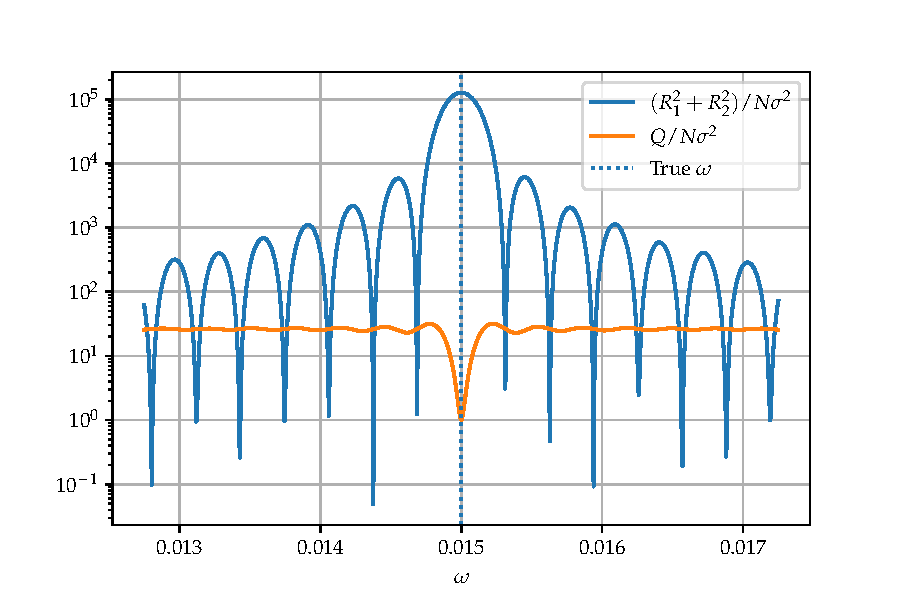
\includegraphics[width=\textwidth]{figures/chisquare_omega.pdf}
\caption{\(N\) data points \(d_i\) are generated with the same distribution as the theoretical model (see figure \ref{fig:signal}). The value of \(Q\) is computed by fixing \(B_1 \) and \(B_2 \) to their true values, which is why its extremal point is sharper: it assumes more knowledge than the alternative, which is what we must maximize after we marginalize over all possible amplitudes \(B_{1, 2}\). }
\label{fig:chisquare_omega}
\end{figure}

As is shown in figure \ref{fig:chisquare_omega}, the maximum of \(R_1^2 + R_2^2\) and the minimum of \(Q\) do indeed coincide. In fact, \(Q\) can also be computed for different values of \(B_1 \) and \(B_2 \), and it attains its global minimum near the true values of the whole triple \((\omega , B_1 , B_2 )\).

This procedure would yield a Gaussian likelihood for \(\omega \) under the following (sufficient) conditions: 
\begin{enumerate}
    \item i.i.d.\ Gaussian noise on each data point;
    \item linear dependence of the model \(f(t)\) on its parameter \(\omega \).
\end{enumerate}

The first condition is satisfied under our hypotheses, the second is not unless the entire data range lies in a very small region: \(N \Delta  \ll \omega^{-1}\), in which case the model can be approximated to linear order; for example, if the region is near the origin we can approximate it as \(f(t) \sim B_1 + B_2 \omega t\).

In the general (and typical) case, instead, the likelihood \(\mathscr{L} \propto \exp(- Q / \sigma^2)\) is not Gaussian, and the model is not linear; however the minimum of \(Q\) is still rather peaked, and as long as we start near it we can numerically find the MAP, or equivalently least-squares, estimate of \(\omega \). 

\end{document}
